\documentclass[a4paper]{book}
\usepackage[utf8]{inputenc}
\usepackage[hidelinks]{hyperref}
\usepackage{pdfpages}
\usepackage{fullpage}
\usepackage{fancyhdr}
\usepackage{xcolor}
\usepackage{graphicx}
\usepackage{wrapfig}
\usepackage{baskervald}
\usepackage{geometry}
\usepackage{multicol}
\fancyhead{}
\fancyfoot[LE,RO]{\thepage}
\cfoot{}
\fancyfoot[LO,RE]{The miniKanren and Relational Programming Workshop 2019}
\renewcommand{\headrulewidth}{0.0pt}
\date{August 22, 2019}
\author{William E. Byrd \and Nada Amin}
\begin{document}
\frontmatter
\setcounter{page}{3}  % cover page to be added by TR editor
\newgeometry{textheight=8.5in,hmargin=20mm}
\chapter*{Preface}
This report aggregates the papers presented at the first miniKanren
and Relational Programming Workshop, hosted on August 2nd, 2019 in
Berlin, Germany and co-located with the twenty-second International
Conference on Functional Programming.

\vspace{5pt}
\noindent
The miniKanren and Relational Programming Workshop is a new workshop for the miniKanren family of relational (pure constraint logic programming) languages: miniKanren, microKanren, core.logic, OCanren, Guanxi, etc. The workshop solicits papers and talks on the design, implementation, and application of miniKanren-like languages. A major goal of the workshop is to bring together researchers, implementors, and users from the miniKanren community, and to share expertise and techniques for relational programming. Another goal for the workshop is to push the state of the art of relational programming—for example, by developing new techniques for writing interpreters, type inferencers, theorem provers, abstract interpreters, CAD tools, and other interesting programs as relations, which are capable of being “run backwards,” performing synthesis, etc.

\vspace{5pt}
\noindent
6 papers were submitted to the workshop, and each submission was reviewed by
two to three members of the program committee.  After deliberation, all submissions
were accepted to the workshop.

\vspace{5pt}
\noindent
In addition to the six full papers  presented
\begin{itemize}
\item William E. Byrd gave a morning tutorial on miniKanren,
\item Daniel P. Friedman and William E. Byrd gave a closing Q\&A with audience.
\end{itemize}

\vspace{5pt}
\noindent
Thanks to all presenters, participants, and members of the
program committee.

\ \\

\ \ \ \ \ \ \ William E. Byrd \& Nada Amin

\ \\

\section*{Program Committee}
\noindent
Claire Alvis, Sparkfund\\
Nada Amin, Harvard University (Program Chair)\\
Tom Gilray, University of Alabama at Birmingham\\
Jason Hemann, Northeastern University\\
Eric Holk, Google\\
Kanae Tsushima, National Institute of Informatics\\
William E. Byrd, University of Alabama at Birmingham (General Chair)\\

\tableofcontents
\mainmatter
\newgeometry{textheight=9.5in,hmargin=20mm}

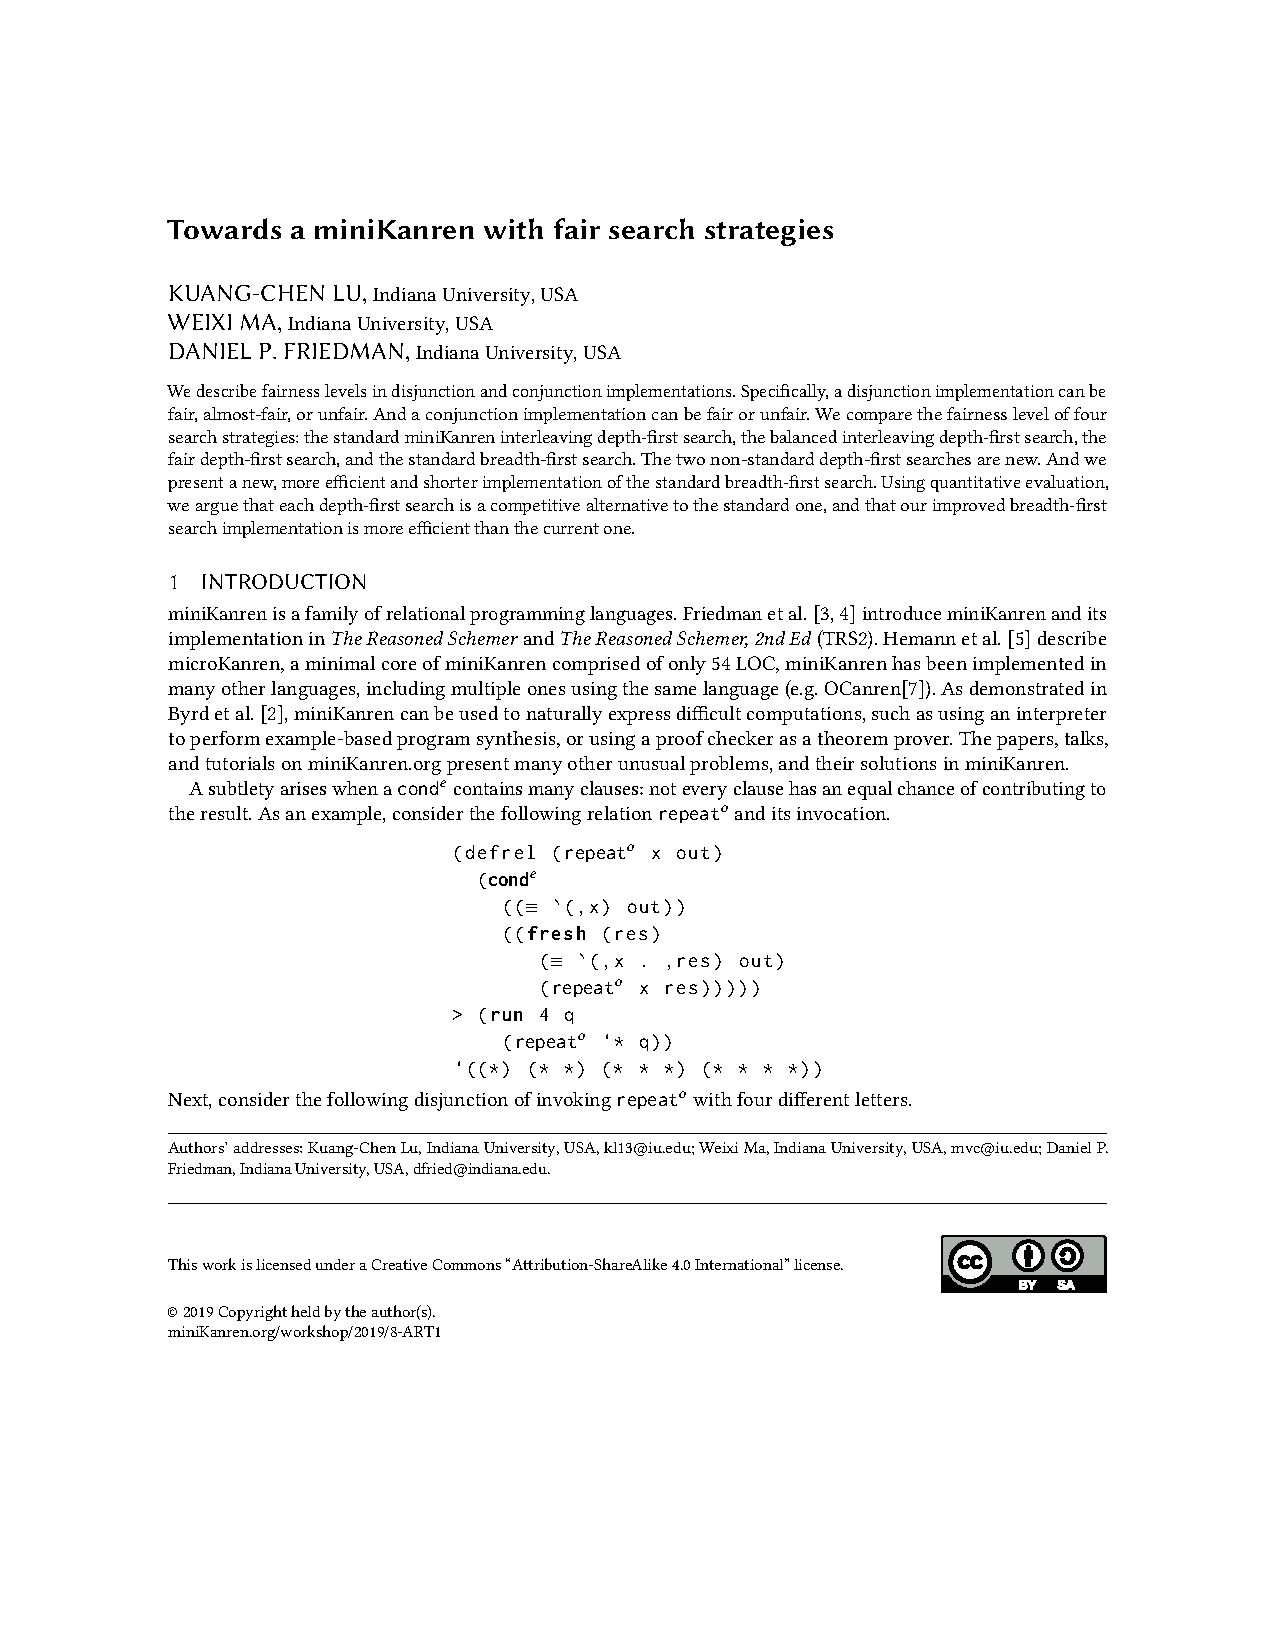
\includepdf[noautoscale,scale=1.07,pages=-,pagecommand={\thispagestyle{fancy}},addtotoc={1,chapter,1,{Towards a miniKanren with fair search strategies by Lu, Ma \& Friedman},p1}]{minikanren19-final1}

\ \\
\pagebreak

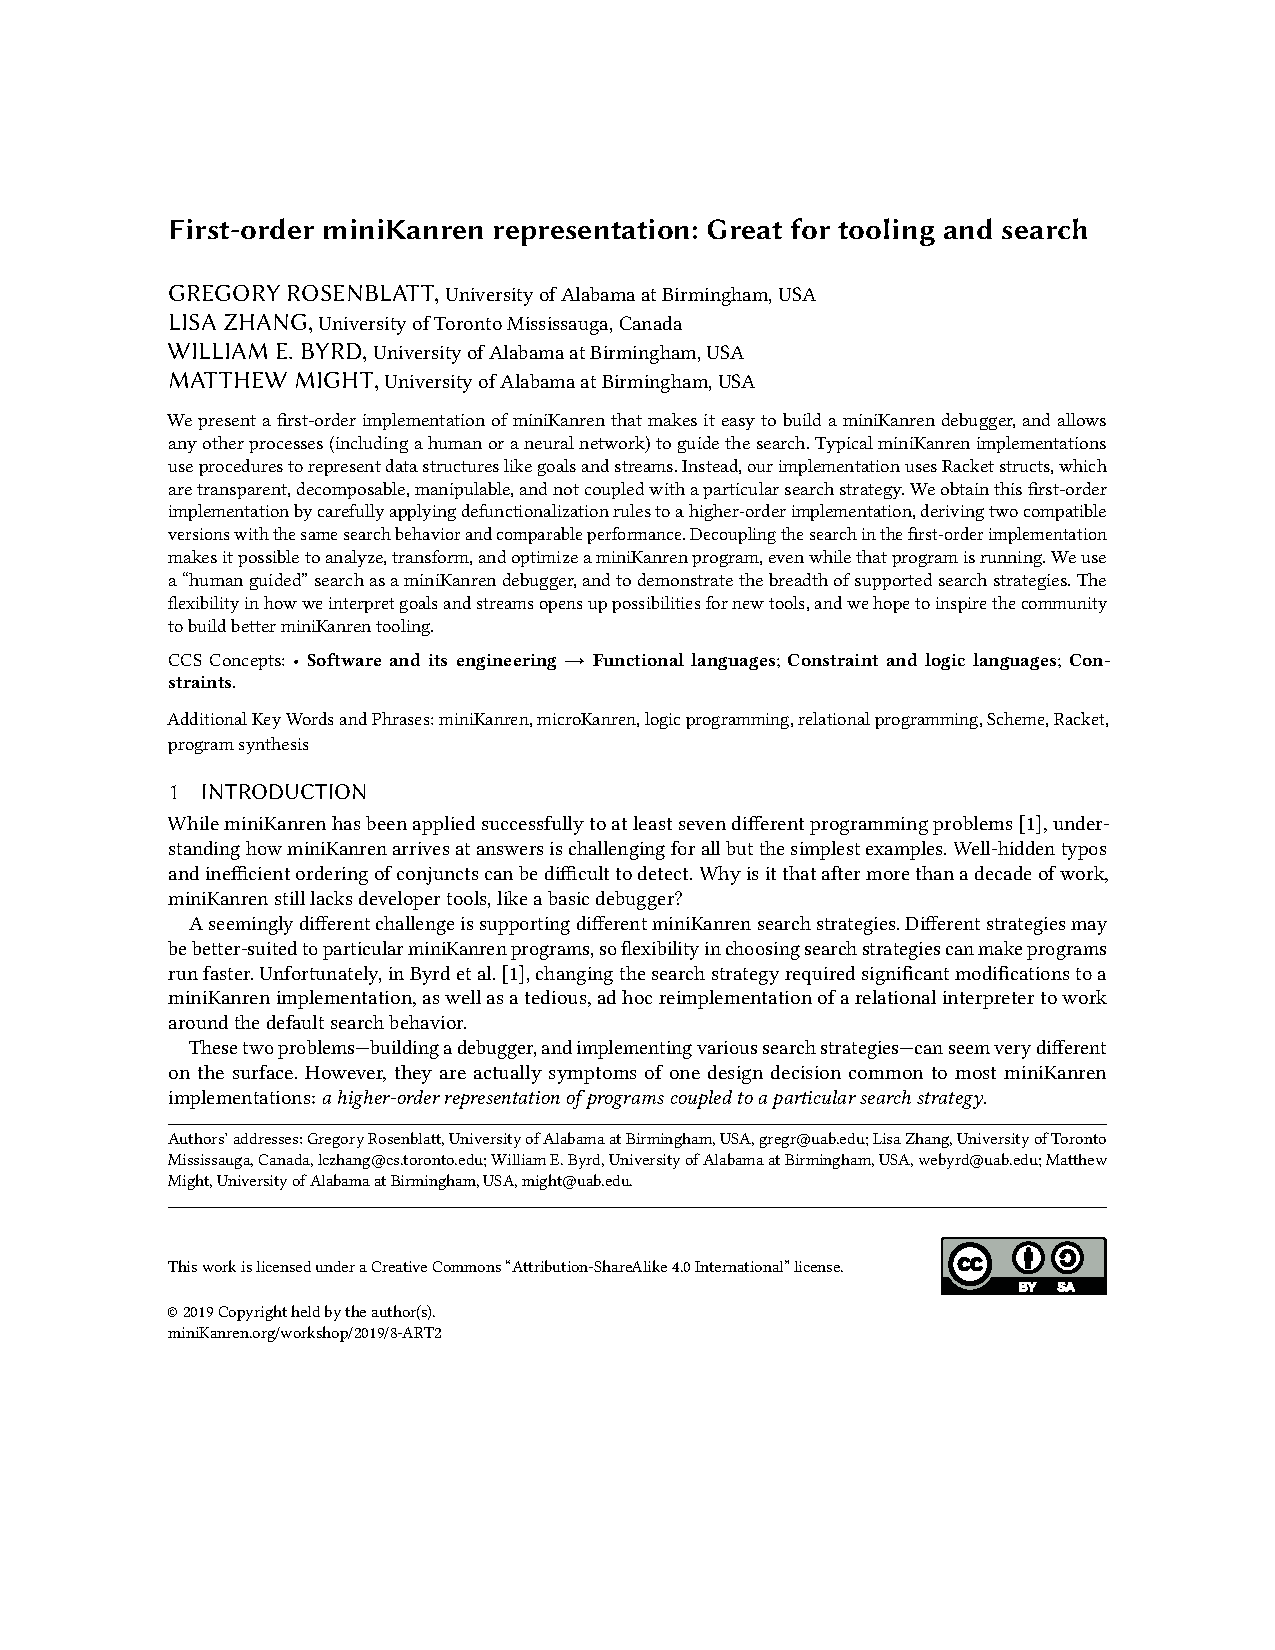
\includepdf[noautoscale,scale=1.07,pages=-,pagecommand={\thispagestyle{fancy}},addtotoc={1,chapter,2,{First-order miniKanren representation by Rosenblatt, Zhang, Byrd \& Might},p2}]{minikanren19-final2}

\ \\
\pagebreak

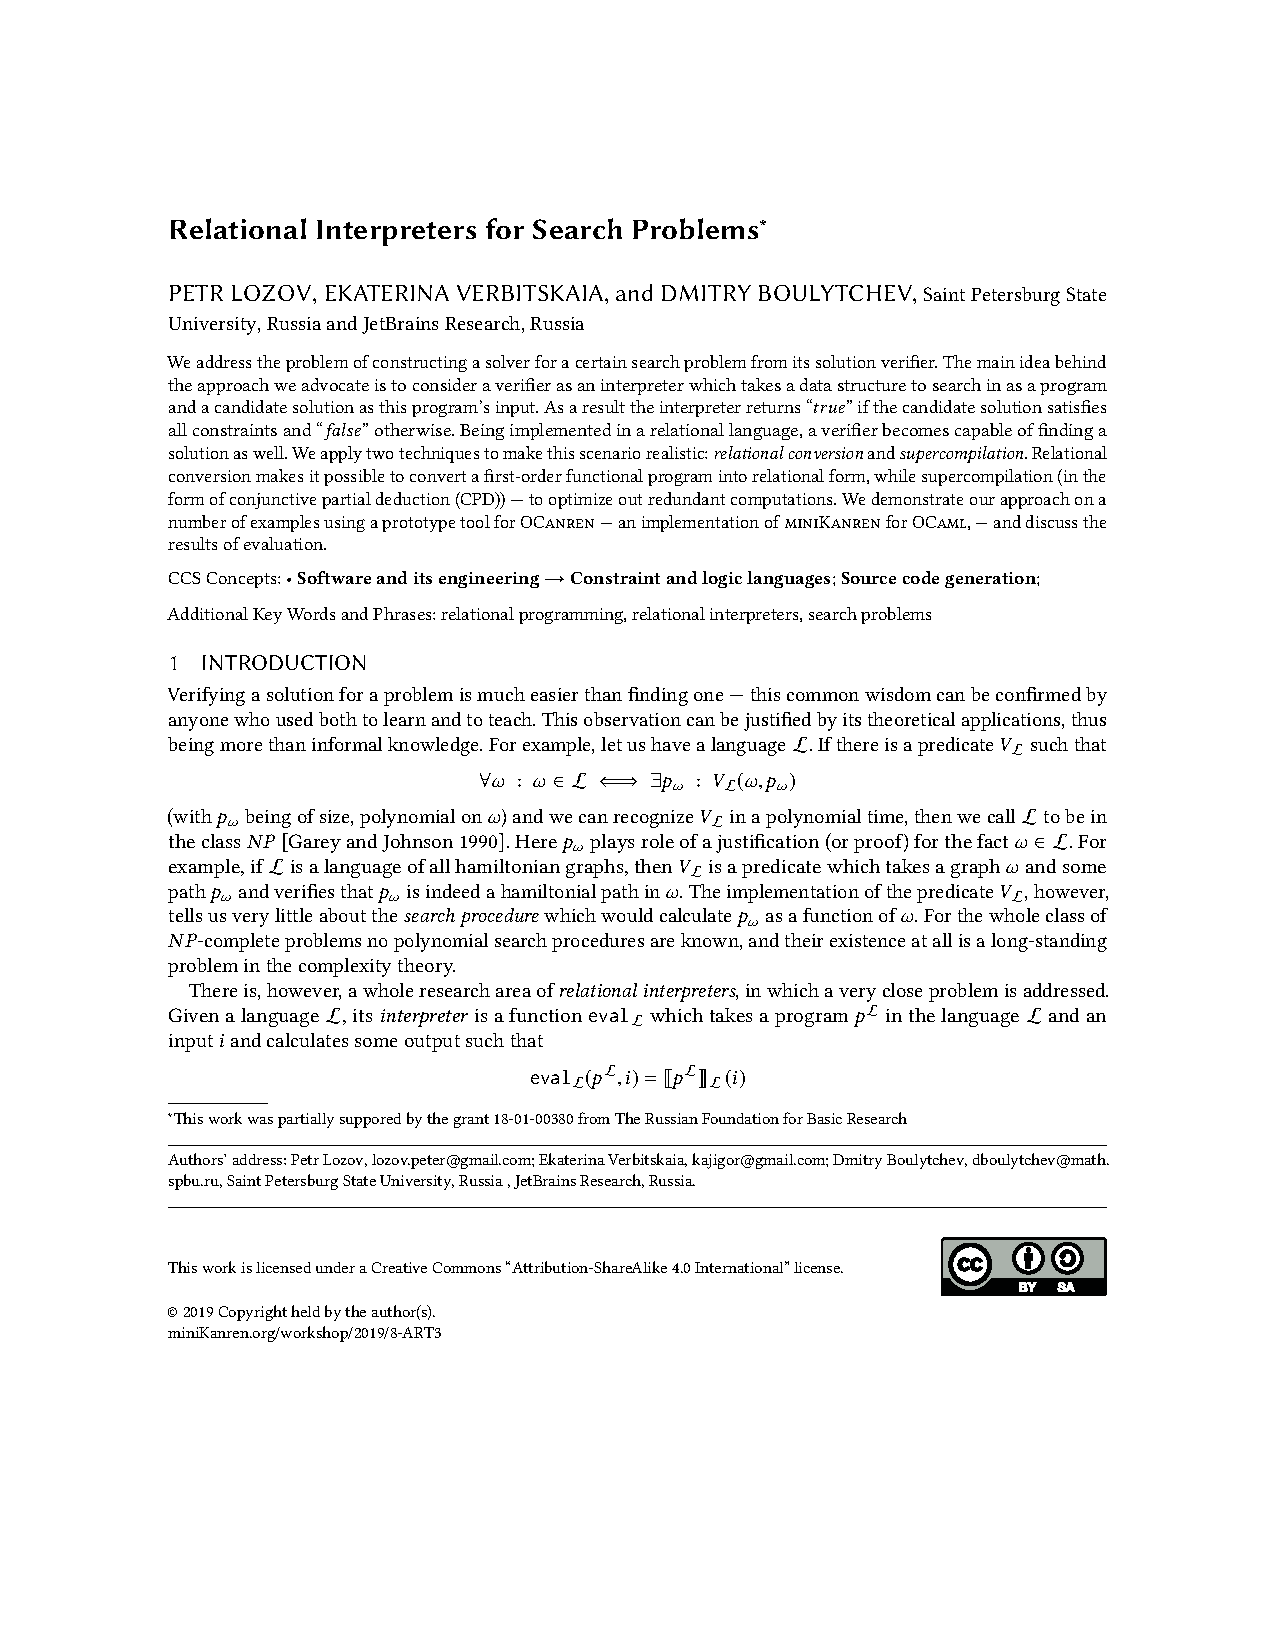
\includepdf[noautoscale,scale=1.07,pages=-,pagecommand={\thispagestyle{fancy}},addtotoc={1,chapter,3,{Relational Interpreters for Search Problems by Lozov, Verbitskaia \& Boulytchev},p3}]{minikanren19-final3}

\ \\
\pagebreak

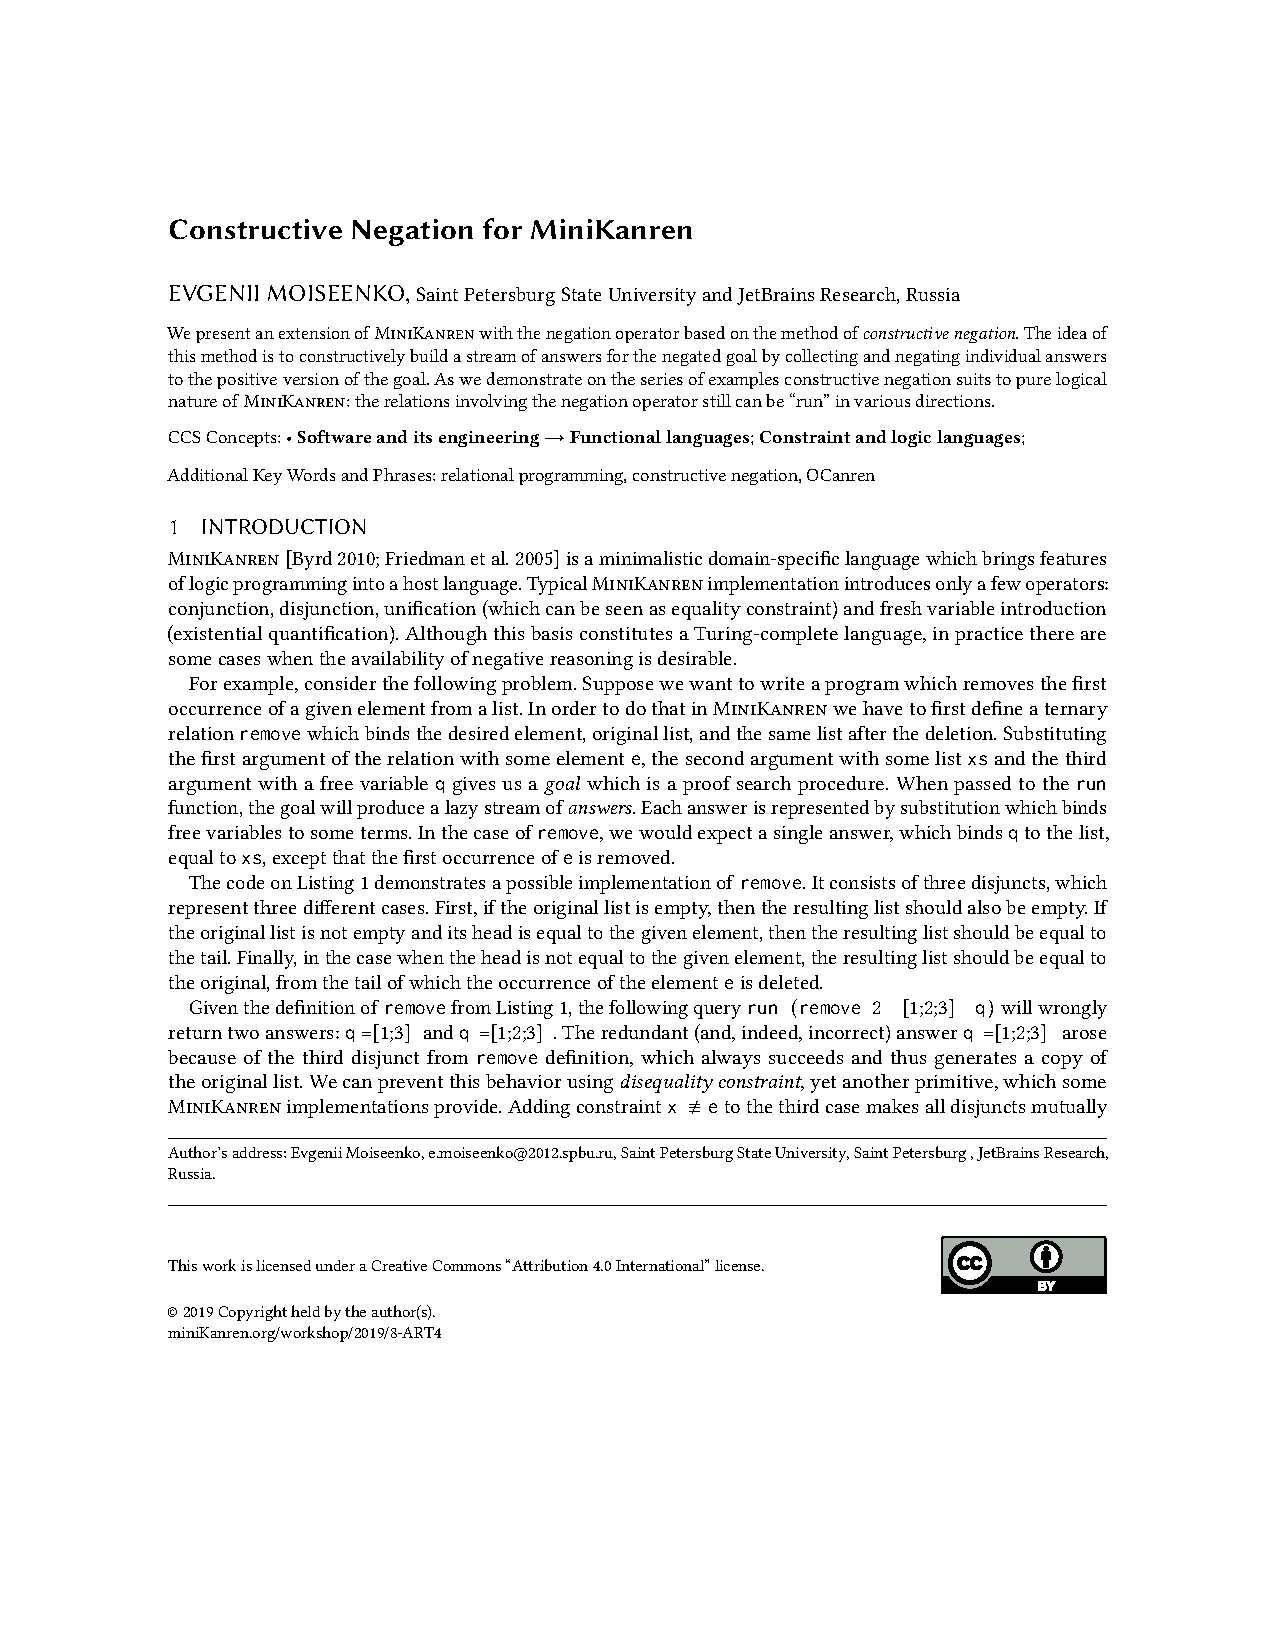
\includepdf[noautoscale,scale=1.07,pages=-,pagecommand={\thispagestyle{fancy}},addtotoc={1,chapter,4,{Constructive Negation for miniKanren by Moiseenko},p4}]{minikanren19-final4}

\ \\
\pagebreak

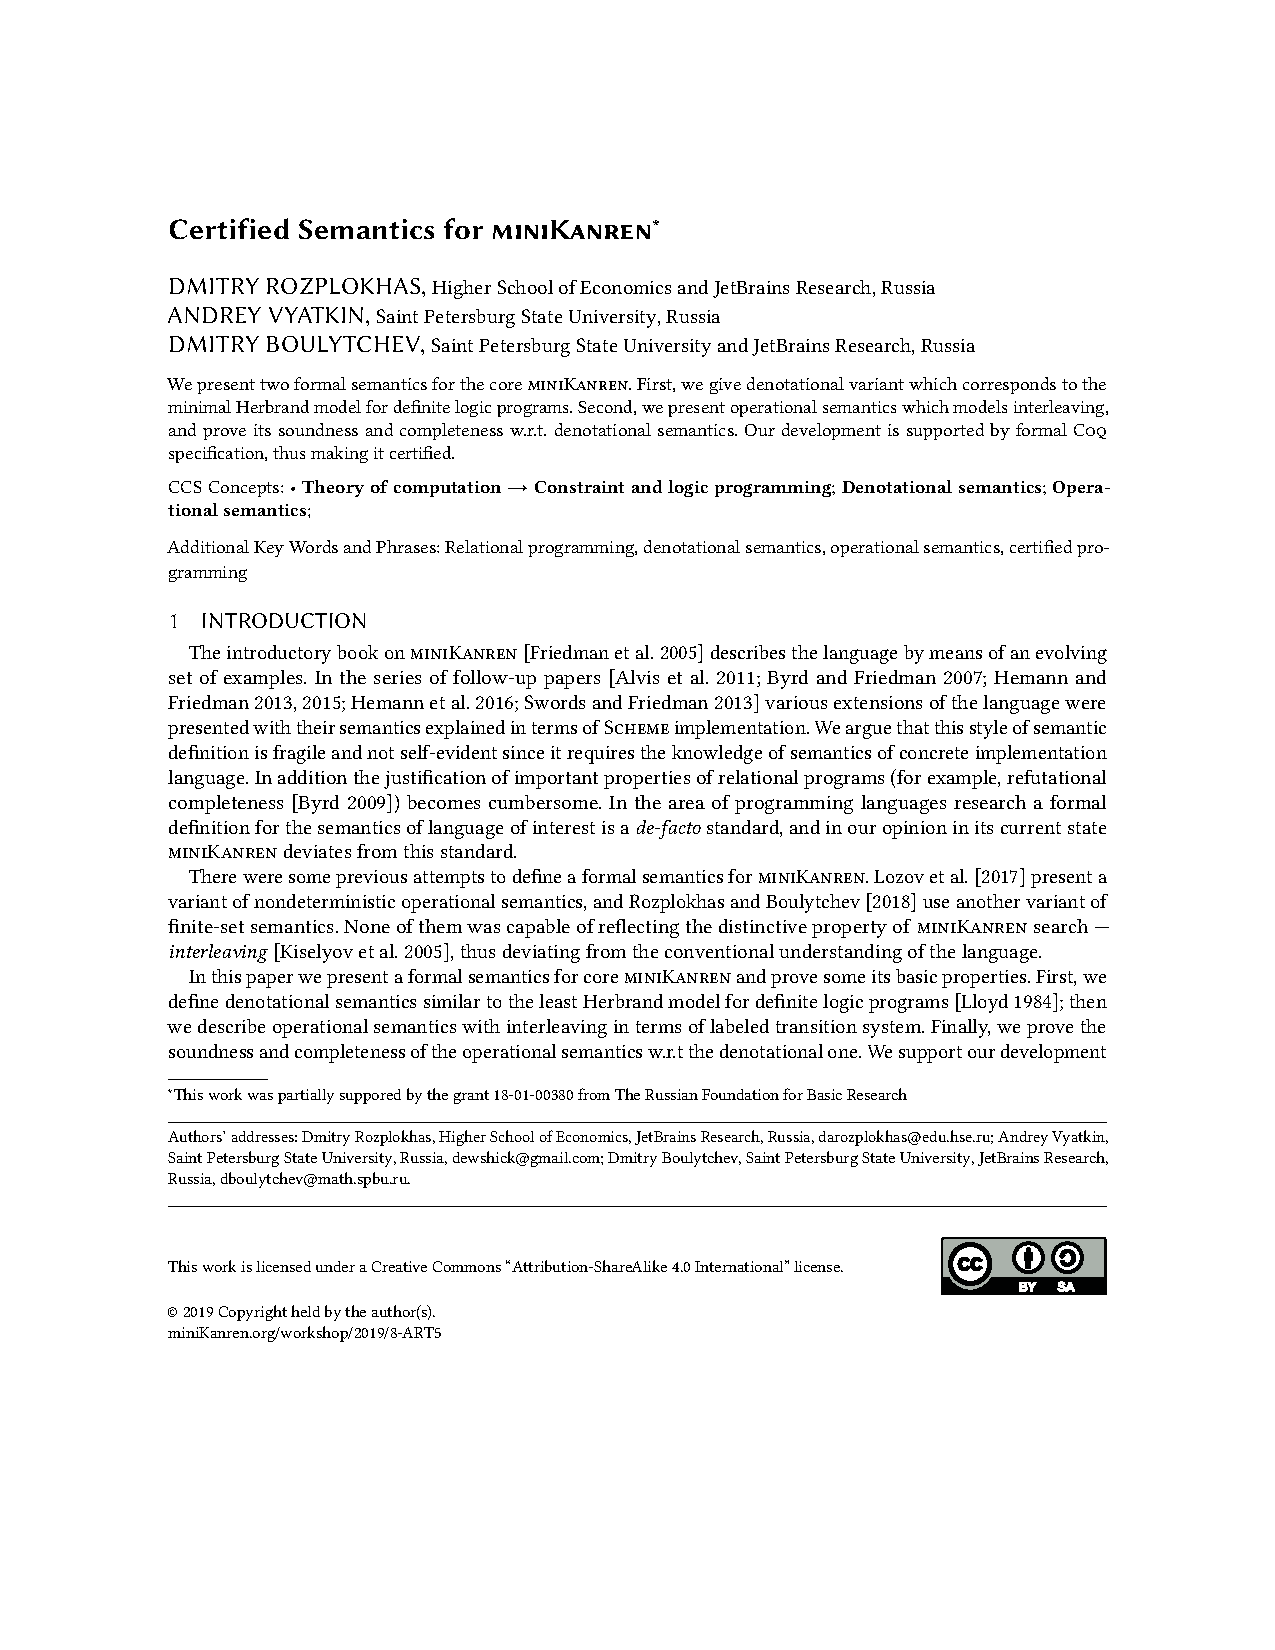
\includepdf[noautoscale,scale=1.07,pages=-,pagecommand={\thispagestyle{fancy}},addtotoc={1,chapter,5,{Certified Semantics for miniKanren by Rozplokhas, Vyatkin \& Boulytchev},p5}]{minikanren19-final5}

\ \\
\pagebreak

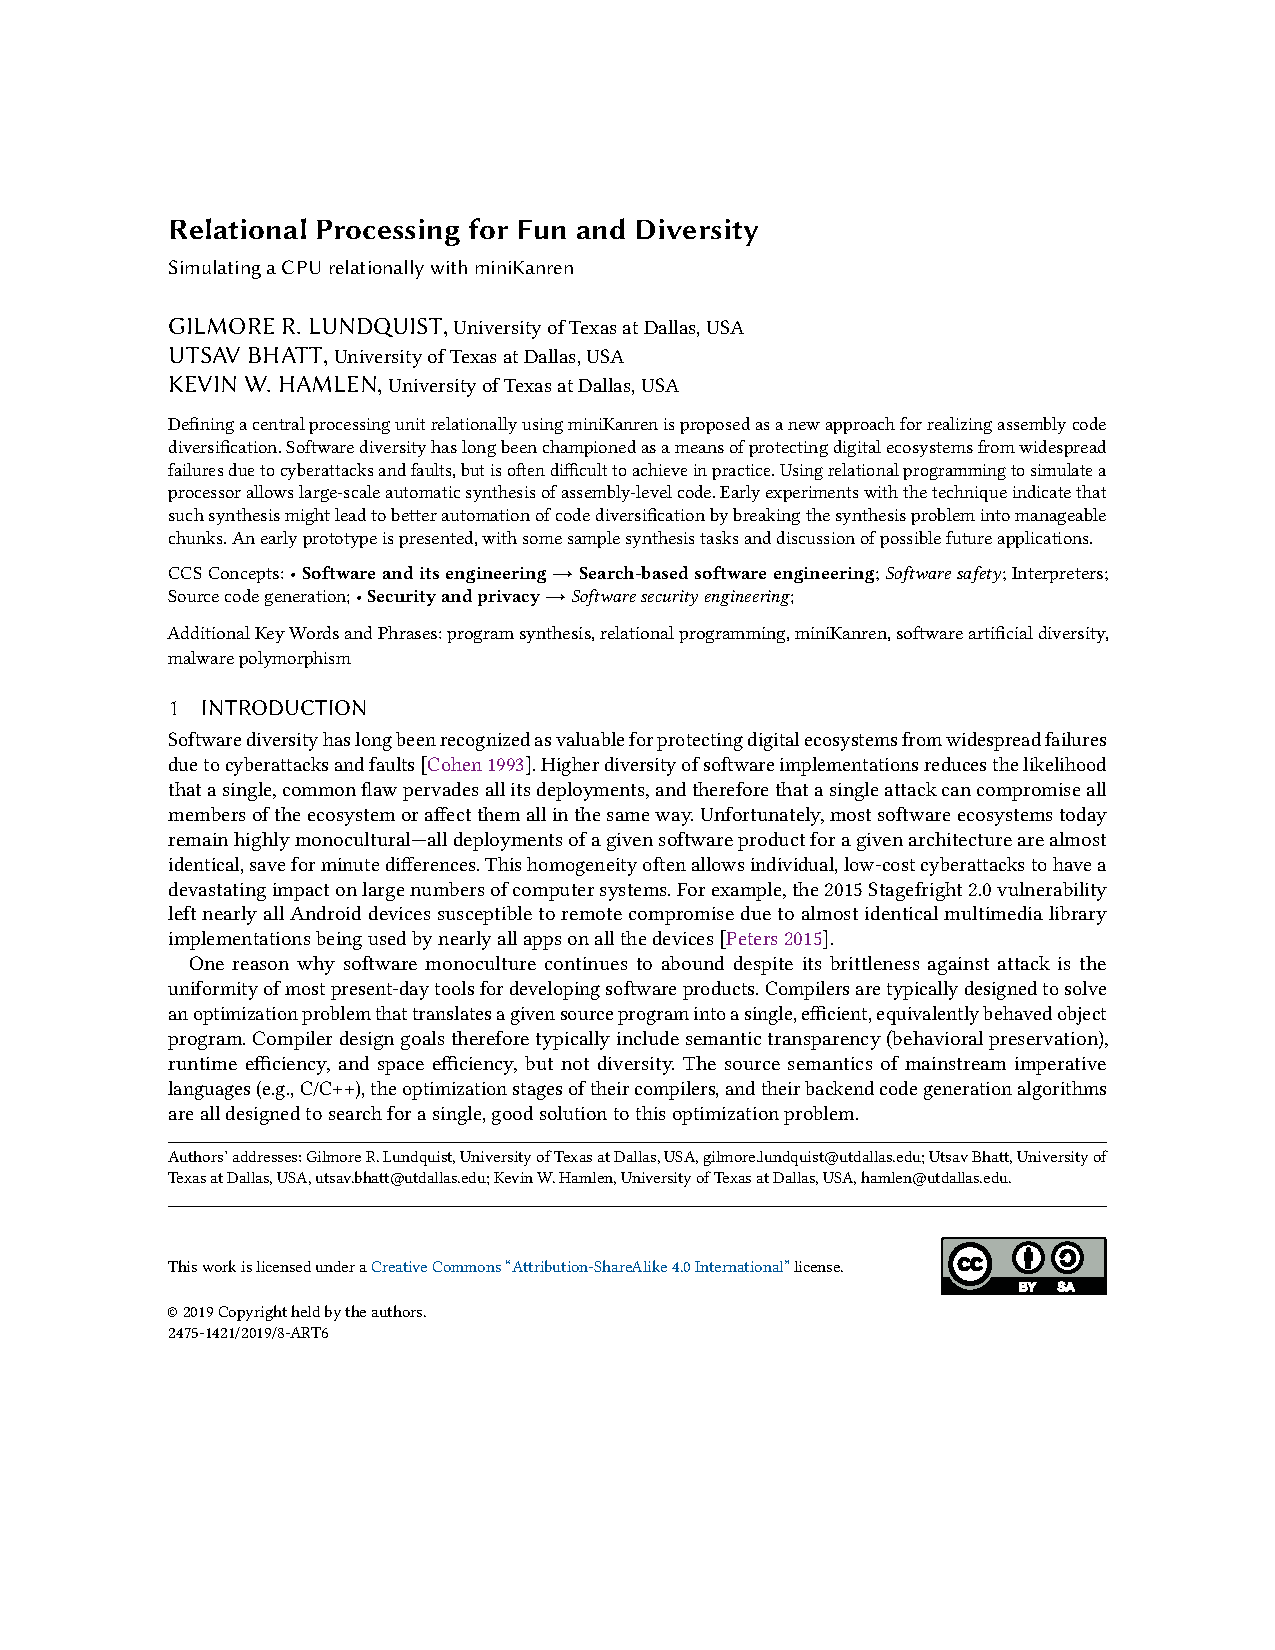
\includepdf[noautoscale,scale=1.07,pages=-,pagecommand={\thispagestyle{fancy}},addtotoc={1,chapter,6,{Relational Processing for Fun and Diversity by Lundquist, Bhatt \& Hamlen},p6}]{minikanren19-final6}

\ \\
\pagebreak

\end{document}
